\documentclass[12pt,a4paper]{article}

% ----------------------------------------------------
% Packages
% ----------------------------------------------------
\usepackage[a4paper,margin=1in]{geometry}
\usepackage{graphicx}
\usepackage{booktabs}
\usepackage{longtable}
\usepackage{tabularx}
\usepackage{array}
\usepackage{float}
\usepackage{enumitem}
\usepackage{setspace}
\usepackage{xcolor}
\usepackage{hyperref}
\usepackage{titlesec}
\usepackage{fancyhdr}
\usepackage{tikz}
\usetikzlibrary{positioning,shapes,arrows.meta}

% ----------------------------------------------------
% Document Formatting
% ----------------------------------------------------

\setstretch{1.5}

\hypersetup{
    colorlinks=true,
    linkcolor=blue,
    urlcolor=blue
}

% ----------------------------------------------------
% Header and Footer
% ----------------------------------------------------

\pagestyle{fancy}
\fancyhf{}

\fancyhead[L]{Dikaios Amanah}
\fancyhead[R]{Software Requirements Specification}

\fancyfoot[C]{\thepage}

% ----------------------------------------------------
% Section Formatting
% ----------------------------------------------------

\titleformat{\section}
{\Large\bfseries}
{\thesection.}{0.5em}{}

\titleformat{\subsection}
{\large\bfseries}
{\thesubsection}{0.5em}{}

% ----------------------------------------------------
% Document
% ----------------------------------------------------

\begin{document}

% ====================================================
% COVER PAGE
% ====================================================

\begin{titlepage}

\centering

\vspace*{1.5cm}

{\Huge\bfseries Dikaios Amanah\par}

\vspace{0.4cm}

{\Large
A Secure, Transparent and Ethical SME Investment Platform\\
Based on Musharakah Principles
}

\vspace{1cm}


\includegraphics[width=0.35\textwidth]{images/uits.png}

\vspace{1cm}

{\Large\bfseries Software Requirements Specification}

\vspace{1.2cm}

Submitted By

\vspace{0.3cm}

{\Large Mehedi Hassan Bhuiyan}

\vspace{0.8cm}

Department of Computer Science and Engineering

University of Information Technology and Sciences (UITS)

\vfill

Submitted To

\vspace{0.3cm}

Dr. Mahfida Amjad Dipa

Software Project Design and Development

\vfill

Academic Year

2026

\end{titlepage}

% ====================================================
% TABLE OF CONTENTS
% ====================================================

\newpage

\tableofcontents

\newpage

% ====================================================
% 1. INTRODUCTION
% ====================================================

\section{Introduction}
\subsection{Purpose}

This Software Requirements Specification (SRS) defines the requirements of
Dikaios Amanah, a secure, transparent, and ethically governed web-based
platform designed to connect Small and Medium Enterprises (SMEs) with
potential investors through a structured investment process.

The purpose of this document is to establish a clear and detailed
specification of the system's expected behavior, functional capabilities,
non-functional requirements, user interactions, data requirements, system
constraints, and testing requirements. The SRS will serve as the primary
reference for the design, development, testing, and evaluation of the
Dikaios Amanah system.

The system is designed around the Musharakah partnership model, where
investment participants share profits and losses according to mutually
agreed terms. The proposed platform emphasizes transparency, verification,
security, and traceability throughout the investment lifecycle.


\subsection{Scope}

Dikaios Amanah will provide a web-based environment through which verified
business owners can present eligible SME investment opportunities and
investors can review and participate in those opportunities.

The system will support three primary user roles:

\begin{itemize}
    \item Business Owner
    \item Investor
    \item Administrator
\end{itemize}

Business owners will be able to create and manage business profiles,
submit required verification information, upload supporting documents,
create investment campaigns after approval, provide business progress
information, and manage campaign-related information.

Investors will be able to create accounts, complete the required
verification process, browse approved investment campaigns, review
business and campaign information, participate in simulated investment
transactions, and monitor their investment portfolio and history.

Administrators will be responsible for platform-level management activities
including user verification, business approval, document review, campaign
moderation, risk assessment, user management, and monitoring of system
activity.

The system will also provide an audit and trust mechanism for important
system events. The proposed architecture includes a Permissioned Trust and
Audit Layer intended to improve transparency and provide tamper-evident
records of critical activities.

The Minimum Viable Product (MVP) will focus on the core platform workflow
required for academic demonstration and evaluation. Real banking
integration, live payment processing, production-level regulatory
implementation, AI-based fraud detection, AI-powered risk prediction,
production Hyperledger Fabric deployment, and automated smart-contract
execution are outside the scope of the MVP.


\subsection{Intended Audience}

This document is intended for the following audiences:

\begin{itemize}
    \item Project developer and system designer
    \item Software Engineering course instructor and evaluator
    \item Software testing and quality assurance personnel
    \item Project stakeholders
    \item Future developers who may extend the system
\end{itemize}

The document provides the requirements and technical specifications needed
to understand the expected behavior and structure of the proposed system.


\subsection{Product Overview}

Dikaios Amanah is intended to function as a technology-enabled platform
connecting verified SMEs seeking investment with verified investors seeking
structured partnership-based investment opportunities.

The proposed system follows the Musharakah principle rather than
interest-based lending. The platform is designed to provide a transparent
investment lifecycle beginning with registration and verification and
continuing through campaign approval, investment participation, agreement
management, business reporting, profit declaration, and profit
distribution.

The system architecture proposed in the project consists of a web
frontend, backend services, a relational database, secure document
storage, authentication and security mechanisms, and a Permissioned Trust
and Audit Layer.

The application layer is planned around React for frontend development and
Node.js with Express.js for backend services. PostgreSQL will be used for
relational data management, while Firebase Storage is intended for secure
document storage. Authentication and authorization mechanisms will protect
user accounts and role-specific functionality.

Critical events and records will be subject to audit mechanisms so that
important activities can be reviewed by authorized users. The trust and
audit mechanism is intended to complement the primary application database
rather than replace it.


\subsection{Definitions and Acronyms}

\begin{description}

    \item[SME] Small and Medium Enterprise.

    \item[MVP] Minimum Viable Product.

    \item[KYC] Know Your Customer.

    \item[RBAC] Role-Based Access Control.

    \item[JWT] JSON Web Token.

    \item[API] Application Programming Interface.

    \item[HTTPS] Hypertext Transfer Protocol Secure.

    \item[SHA-256] Secure Hash Algorithm 256-bit.

    \item[SRS] Software Requirements Specification.

    \item[UML] Unified Modeling Language.

    \item[SDLC] Software Development Life Cycle.

    \item[ERD] Entity Relationship Diagram.

\end{description}


\subsection{References}

The primary project-specific source for this Software Requirements
Specification is the Dikaios Amanah Project Proposal. The proposal
establishes the project's background, objectives, scope, proposed solution,
system architecture, technology stack, feasibility considerations,
limitations, and planned development activities.

Additional technical and domain references are listed in the References
section of this document.


% ====================================================
% 2. OVERALL DESCRIPTION
% ====================================================

\IfFileExists{chapters/overall_description.tex}{
    \section{Overall Description}
    \subsection{Product Perspective}

Dikaios Amanah is a web-based software platform designed to facilitate
structured interaction between verified Small and Medium Enterprises (SMEs),
retail investors, and system administrators.

The system follows a layered three-tier architecture consisting of a
presentation layer, an application layer, and a data layer. The separation
of these layers allows user interaction, application logic, security
controls, and persistent data management to be handled independently.

The presentation layer provides the web interface for Business Owners,
Investors, and Administrators. The application layer processes requests,
enforces business rules, manages authentication and authorization, and
coordinates the major platform services. The data layer manages operational
records, business information, investment information, and supporting
documents.

The proposed system is intended to operate as a technology-enabled
intermediary rather than as a financial institution. Investment transactions
within the academic MVP will be simulated for demonstration and testing
purposes.


\subsection{Product Functions}

The major functions of Dikaios Amanah are organized according to the
responsibilities of the system's primary users.

\subsubsection{User Registration and Authentication}

The system will provide account registration and authentication mechanisms
for users. Authentication will use secure password handling and token-based
session management. Access to system resources will be controlled according
to the user's assigned role.

\subsubsection{Business Owner Functions}

Business Owners will be able to:

\begin{itemize}
    \item Register an account.
    \item Complete identity and business verification.
    \item Manage business profile information.
    \item Submit supporting documents.
    \item Create investment campaigns after approval.
    \item Monitor campaign progress.
    \item Provide business progress information.
    \item Declare business profits.
    \item Communicate relevant information to investors.
\end{itemize}

A business must complete the required verification and administrative review
before its investment campaign becomes available to investors.


\subsubsection{Investor Functions}

Investors will be able to:

\begin{itemize}
    \item Register an account.
    \item Complete the required KYC verification process.
    \item Discover verified businesses and approved campaigns.
    \item Review business and campaign information.
    \item Review available risk information.
    \item Participate in simulated investment transactions.
    \item Monitor investments.
    \item View portfolio information.
    \item Track investment history.
    \item Monitor declared profits.
\end{itemize}


\subsubsection{Administrator Functions}

Administrators will be responsible for maintaining platform integrity and
managing operational activities. Administrative functions will include:

\begin{itemize}
    \item User verification.
    \item Business approval and rejection.
    \item Document validation.
    \item Risk assessment management.
    \item Campaign moderation.
    \item User management.
    \item Audit monitoring.
    \item Platform activity monitoring.
    \item Platform reporting.
\end{itemize}

Administrative actions will be recorded through the system's activity and
audit mechanisms.


\subsubsection{Investment Campaign Management}

The system will allow approved Business Owners to create and manage
investment campaigns. Campaign information will be presented to Investors
after the required administrative approval.

Investors will be able to review approved campaigns before participating.
The campaign lifecycle will support the proposed workflow from campaign
publication through investment participation and eventual completion.


\subsubsection{Document Management}

The system will allow Business Owners to submit supporting documents during
the verification process. Documents will be stored using the planned secure
cloud storage mechanism.

Cryptographic hashing will be used to support document integrity
verification and help identify unauthorized modification of stored
document
content.


\subsubsection{Trust and Audit Functions}

The system will maintain records of important platform events through a
Permissioned Trust and Audit Layer.

Critical events identified by the project proposal include:

\begin{itemize}
    \item Business verification.
    \item Contract approval.
    \item Investment confirmation.
    \item Profit declaration.
    \item Audit records.
    \item Document integrity verification.
\end{itemize}

The trust and audit mechanism will complement the primary relational
database rather than replace it.


\subsubsection{Notification and Activity Functions}

The system will provide notifications and activity information to help
users remain aware of relevant actions and changes within the platform.

Examples include verification status changes, campaign-related updates,
investment-related activities, and administrative actions.


\subsection{User Classes and Characteristics}

Dikaios Amanah contains three primary user classes.

\subsubsection{Business Owner}

A Business Owner represents an SME seeking investment through the platform.
Business Owners are expected to provide accurate business information and
supporting documentation. They will primarily interact with the platform
through the Business Owner Dashboard.

\subsubsection{Investor}

An Investor represents an individual seeking to participate in verified
Musharakah-based investment opportunities. Investors will use the platform
to review business information, evaluate available opportunities, manage
simulated investments, and monitor their portfolios.

\subsubsection{Administrator}

An Administrator is an authorized platform operator responsible for
verification, approval, monitoring, moderation, and other administrative
activities. Administrators have access to functions that are restricted
from Business Owners and Investors.


\subsection{Operating Environment}

The proposed system will operate as a web-based application.

The planned software environment consists of:

\begin{itemize}
    \item React.js for the frontend application.
    \item Node.js as the backend runtime environment.
    \item Express.js for backend and RESTful API services.
    \item PostgreSQL for relational data management.
    \item Firebase Storage for secure document storage.
    \item JWT for authentication.
    \item bcrypt for password hashing.
    \item SHA-256 for document integrity verification.
    \item Git and GitHub for version control.
\end{itemize}

Users will access the system through modern web browsers using an internet
connection. Communication between the frontend and backend services will
use HTTPS.


\subsection{Design Constraints}

The following constraints are derived from the defined project scope and
academic MVP objectives:

\begin{itemize}
    \item The project must remain within the defined academic MVP scope.
    \item Investment transactions will be simulated rather than connected to
    real financial payment systems.
    \item Live banking integration is excluded from the MVP.
    \item Real payment gateway integration is excluded from the MVP.
    \item Production-level BSEC regulatory compliance implementation is
    excluded from the MVP.
    \item AI-based fraud detection is excluded from the MVP.
    \item AI-powered risk prediction is excluded from the MVP.
    \item Production Hyperledger Fabric deployment is excluded from the MVP.
    \item Automated smart contract execution is excluded from the MVP.
    \item Native Android and iOS applications are excluded from the MVP.
\end{itemize}

These limitations are intended to keep the system technically achievable
within the project's academic development scope.


\subsection{Assumptions and Dependencies}

The system development is based on several assumptions established in the
project proposal:

\begin{itemize}
    \item Users have basic digital literacy.
    \item Users have access to an internet connection.
    \item Businesses provide authentic documentation.
    \item Administrators perform verification activities responsibly.
    \item The system is initially developed for academic demonstration
    purposes.
    \item Investment transactions used during testing are simulated.
\end{itemize}

The system also depends on the availability and proper operation of its
planned software and infrastructure components, including the relational
database, document storage service, authentication mechanisms, and
deployment environment.
}{}

% ====================================================
% 3. FUNCTIONAL REQUIREMENTS
% ====================================================

\IfFileExists{chapters/functional_requirements.tex}{
    \section{Functional Requirements}
    % ====================================================
% 3. Functional Requirements
% ====================================================

\subsection{Authentication and Account Management}

\subsubsection{FR-AUTH-01: User Registration}

The system shall allow a new user to register an account by providing the
required personal and account information.

\subsubsection{FR-AUTH-02: User Login}

The system shall authenticate registered users using their valid login
credentials.

\subsubsection{FR-AUTH-03: Role-Based Access}

The system shall assign users an appropriate system role and restrict access
to functions according to the user's authorized role.

The primary roles shall be:

\begin{itemize}
    \item Business Owner
    \item Investor
    \item Administrator
\end{itemize}

\subsubsection{FR-AUTH-04: Secure Password Storage}

The system shall store user passwords using a secure password-hashing
mechanism rather than storing plaintext passwords.

\subsubsection{FR-AUTH-05: Session Authentication}

The system shall maintain authenticated user sessions using a secure
token-based authentication mechanism.

\subsubsection{FR-AUTH-06: Account Management}

The system shall allow authenticated users to view and manage their
permitted account and profile information.


% ====================================================
% Business Owner Requirements
% ====================================================

\subsection{Business Owner Requirements}

\subsubsection{FR-BUS-01: Business Profile Creation}

The system shall allow an authenticated Business Owner to create a business
profile containing the required business information.

\subsubsection{FR-BUS-02: Business Profile Management}

The system shall allow a Business Owner to update permitted business profile
information.

\subsubsection{FR-BUS-03: Verification Submission}

The system shall allow a Business Owner to submit the required business
verification information for administrative review.

\subsubsection{FR-BUS-04: Document Submission}

The system shall allow a Business Owner to upload supporting documents
required for the verification process.

\subsubsection{FR-BUS-05: Verification Status}

The system shall allow a Business Owner to view the current status of the
business verification process.

\subsubsection{FR-BUS-06: Campaign Creation}

The system shall allow an approved Business Owner to create an investment
campaign containing the required campaign information.

\subsubsection{FR-BUS-07: Campaign Management}

The system shall allow an authorized Business Owner to view and manage
permitted information associated with their campaigns.

\subsubsection{FR-BUS-08: Campaign Progress}

The system shall allow a Business Owner to monitor the funding progress of
an approved campaign.

\subsubsection{FR-BUS-09: Business Progress Reporting}

The system shall allow a Business Owner to submit business progress
information relevant to an active campaign.

\subsubsection{FR-BUS-10: Profit Declaration}

The system shall allow an authorized Business Owner to record declared
business profit information associated with an investment campaign.


% ====================================================
% Investor Requirements
% ====================================================

\subsection{Investor Requirements}

\subsubsection{FR-INV-01: Investor Verification}

The system shall allow an Investor to submit the required information for
the investor verification process.

\subsubsection{FR-INV-02: Investor Dashboard}

The system shall provide an authenticated Investor with a dashboard
containing relevant investment and account information.

\subsubsection{FR-INV-03: Campaign Discovery}

The system shall allow verified Investors to browse approved investment
campaigns.

\subsubsection{FR-INV-04: Campaign Information}

The system shall allow an Investor to view relevant information about an
approved investment campaign before participating.

\subsubsection{FR-INV-05: Business Information}

The system shall allow an Investor to view permitted information about the
business associated with an approved investment campaign.

\subsubsection{FR-INV-06: Risk Information}

The system shall present available risk assessment information associated
with an investment opportunity.

\subsubsection{FR-INV-07: Simulated Investment}

The system shall allow an eligible Investor to participate in a simulated
investment transaction during the MVP.

\subsubsection{FR-INV-08: Investment Confirmation}

The system shall provide confirmation after a simulated investment has been
successfully recorded.

\subsubsection{FR-INV-09: Portfolio Management}

The system shall allow an Investor to view their investment portfolio.

\subsubsection{FR-INV-10: Investment History}

The system shall allow an Investor to view the history of their recorded
investment activities.

\subsubsection{FR-INV-11: Profit Information}

The system shall allow an Investor to view declared profit information
associated with their investments.


% ====================================================
% Administrator Requirements
% ====================================================

\subsection{Administrator Requirements}

\subsubsection{FR-ADMIN-01: Administrator Dashboard}

The system shall provide an authenticated Administrator with an
administrative dashboard containing relevant platform information.

\subsubsection{FR-ADMIN-02: User Management}

The system shall allow authorized Administrators to view and manage user
accounts according to their administrative permissions.

\subsubsection{FR-ADMIN-03: Business Verification Review}

The system shall allow an Administrator to review submitted business
verification information.

\subsubsection{FR-ADMIN-04: Business Approval}

The system shall allow an Administrator to approve or reject a business
verification request.

\subsubsection{FR-ADMIN-05: Document Review}

The system shall allow an Administrator to review documents submitted as
part of the verification process.

\subsubsection{FR-ADMIN-06: Risk Assessment Management}

The system shall allow an authorized Administrator to manage the risk
assessment information associated with eligible businesses or campaigns.

\subsubsection{FR-ADMIN-07: Campaign Moderation}

The system shall allow an Administrator to review and moderate submitted
investment campaigns.

\subsubsection{FR-ADMIN-08: Campaign Approval}

The system shall allow an Administrator to approve or reject a submitted
investment campaign.

\subsubsection{FR-ADMIN-09: Platform Activity Monitoring}

The system shall allow an Administrator to monitor relevant platform
activities.

\subsubsection{FR-ADMIN-10: Platform Reporting}

The system shall provide authorized Administrators with access to relevant
platform reports.


% ====================================================
% Campaign Management
% ====================================================

\subsection{Investment Campaign Management}

\subsubsection{FR-CAM-01: Campaign Submission}

The system shall allow an approved Business Owner to submit an investment
campaign for administrative review.

\subsubsection{FR-CAM-02: Campaign Approval Status}

The system shall maintain the approval status of each submitted campaign.

\subsubsection{FR-CAM-03: Campaign Publication}

The system shall make an approved campaign available to eligible Investors.

\subsubsection{FR-CAM-04: Campaign Information Display}

The system shall display the relevant campaign information required for an
Investor to review an investment opportunity.

\subsubsection{FR-CAM-05: Campaign Funding Progress}

The system shall maintain and display the recorded funding progress of an
active campaign.

\subsubsection{FR-CAM-06: Campaign Lifecycle}

The system shall maintain the status of a campaign throughout its defined
lifecycle, including relevant approval, active, and completed states.


% ====================================================
% Document Management
% ====================================================

\subsection{Document Management Requirements}

\subsubsection{FR-DOC-01: Document Upload}

The system shall allow authorized users to upload documents required for
verification and other permitted platform activities.

\subsubsection{FR-DOC-02: Secure Document Storage}

The system shall store uploaded documents using the designated secure
document storage service.

\subsubsection{FR-DOC-03: Document Integrity Hash}

The system shall generate a cryptographic hash for applicable uploaded
documents to support document integrity verification.

\subsubsection{FR-DOC-04: Document Verification}

The system shall allow authorized Administrators to review the integrity
information associated with submitted documents.


% ====================================================
% Notification and Activity Requirements
% ====================================================

\subsection{Notification and Activity Requirements}

\subsubsection{FR-NOT-01: User Notifications}

The system shall provide notifications for relevant events affecting
authorized users.

\subsubsection{FR-NOT-02: Verification Notification}

The system shall notify relevant users when the status of a verification
request changes.

\subsubsection{FR-NOT-03: Campaign Notification}

The system shall provide relevant campaign-related activity notifications
to authorized users.

\subsubsection{FR-NOT-04: Activity History}

The system shall maintain a history of relevant user and platform
activities.


% ====================================================
% Trust and Audit Requirements
% ====================================================

\subsection{Trust and Audit Requirements}

\subsubsection{FR-AUD-01: Critical Event Recording}

The system shall record defined critical system events through the
Permissioned Trust and Audit Layer.

\subsubsection{FR-AUD-02: Business Verification Audit}

The system shall record relevant business verification events in the audit
record.

\subsubsection{FR-AUD-03: Contract Approval Audit}

The system shall record relevant contract approval events in the audit
record.

\subsubsection{FR-AUD-04: Investment Confirmation Audit}

The system shall record relevant investment confirmation events in the
audit record.

\subsubsection{FR-AUD-05: Profit Declaration Audit}

The system shall record relevant profit declaration events in the audit
record.

\subsubsection{FR-AUD-06: Audit Record Access}

The system shall allow authorized users to view permitted audit and activity
information.

\subsubsection{FR-AUD-07: Audit Integrity}

The system shall provide a mechanism for detecting unauthorized alteration
of applicable audit records.


% ====================================================
% Agreement and Investment Lifecycle
% ====================================================

\subsection{Investment Lifecycle Requirements}

\subsubsection{FR-LIFE-01: Investment Participation}

The system shall associate a recorded simulated investment with the
corresponding Investor and approved campaign.

\subsubsection{FR-LIFE-02: Investment Record}

The system shall maintain the information necessary to identify a recorded
investment, its associated campaign, and its participating Investor.

\subsubsection{FR-LIFE-03: Profit Record}

The system shall maintain declared profit information associated with
eligible investment activities.

\subsubsection{FR-LIFE-04: Investment Status}

The system shall maintain the status of recorded investment activities
throughout the supported investment lifecycle.
}{}

% ====================================================
% 4. NON-FUNCTIONAL REQUIREMENTS
% ====================================================

\IfFileExists{chapters/non_functional_requirements.tex}{
    \section{Non-Functional Requirements}
    % ====================================================
% 4. Non-Functional Requirements
% ====================================================

\subsection{Security Requirements}

\subsubsection{NFR-SEC-01: Authentication Security}

The system shall require users to authenticate before accessing protected
system functions.

\subsubsection{NFR-SEC-02: Role-Based Authorization}

The system shall restrict access to protected resources according to the
authenticated user's assigned role.

\subsubsection{NFR-SEC-03: Password Protection}

The system shall not store user passwords in plaintext. Passwords shall be
protected using a secure password-hashing mechanism.

\subsubsection{NFR-SEC-04: Secure Communication}

The deployed system shall use HTTPS for communication between clients and
server-side services.

\subsubsection{NFR-SEC-05: Document Integrity}

The system shall use cryptographic hashing to support verification of the
integrity of applicable uploaded documents.

\subsubsection{NFR-SEC-06: Audit Protection}

The system shall provide mechanisms to detect unauthorized alteration of
applicable audit records.

\subsubsection{NFR-SEC-07: Sensitive Data Protection}

The system shall restrict access to sensitive business, investor,
verification, and administrative information to authorized users.


% ====================================================
% Performance Requirements
% ====================================================

\subsection{Performance Requirements}

\subsubsection{NFR-PERF-01: Normal Request Response}

Under the expected workload of the academic MVP, normal user requests
should receive a response within an acceptable period that does not
unnecessarily interrupt the user's workflow.

\subsubsection{NFR-PERF-02: Dashboard Loading}

The system should load normal user dashboard information without excessive
delay under the expected academic demonstration workload.

\subsubsection{NFR-PERF-03: Database Operations}

The system shall use appropriate database queries and indexing strategies
to support efficient retrieval of frequently accessed application data.

\subsubsection{NFR-PERF-04: Document Operations}

Document upload and retrieval operations should provide appropriate
feedback to users while the operation is being processed.


% ====================================================
% Usability Requirements
% ====================================================

\subsection{Usability Requirements}

\subsubsection{NFR-USE-01: Consistent Interface}

The system shall provide a consistent user interface across the major
platform modules.

\subsubsection{NFR-USE-02: Role-Specific Navigation}

The system shall provide navigation appropriate to the authenticated
user's role.

\subsubsection{NFR-USE-03: Form Validation}

The system shall provide appropriate validation and feedback when users
submit forms.

\subsubsection{NFR-USE-04: Error Feedback}

The system shall provide understandable error messages when an operation
cannot be completed.

\subsubsection{NFR-USE-05: Responsive Interface}

The web interface should support common desktop, tablet, and mobile
screen sizes.

\subsubsection{NFR-USE-06: Status Visibility}

The system shall clearly communicate important statuses such as
verification, campaign approval, investment, and other relevant workflow
states.


% ====================================================
% Reliability Requirements
% ====================================================

\subsection{Reliability Requirements}

\subsubsection{NFR-REL-01: Data Consistency}

The system shall maintain consistency between related application records.

\subsubsection{NFR-REL-02: Transaction Integrity}

The system shall ensure that supported investment and other critical
operations either complete successfully or do not leave inconsistent
application records.

\subsubsection{NFR-REL-03: Error Handling}

The system shall handle expected application errors without exposing
sensitive implementation details to users.

\subsubsection{NFR-REL-04: Data Persistence}

Successfully stored application records shall remain available after
normal application sessions have ended.


% ====================================================
% Maintainability Requirements
% ====================================================

\subsection{Maintainability Requirements}

\subsubsection{NFR-MNT-01: Modular Architecture}

The system shall maintain a modular separation between frontend,
backend, database, and supporting services.

\subsubsection{NFR-MNT-02: Source Code Organization}

The source code shall follow a structured organization that allows
individual components to be modified without unnecessary changes to
unrelated components.

\subsubsection{NFR-MNT-03: Version Control}

The project source code and documentation shall be maintained using
version control.

\subsubsection{NFR-MNT-04: Documentation}

Major system components and interfaces shall be documented sufficiently
to support future maintenance and development.

\subsubsection{NFR-MNT-05: Configuration Separation}

Environment-specific configuration and sensitive credentials shall be
kept separate from the application source code.


% ====================================================
% Scalability Requirements
% ====================================================

\subsection{Scalability Requirements}

\subsubsection{NFR-SCL-01: Modular Expansion}

The architecture should allow additional platform features to be added
without requiring a complete redesign of the existing system.

\subsubsection{NFR-SCL-02: User Growth}

The system architecture should allow the number of users and application
records to increase beyond the initial academic demonstration workload.

\subsubsection{NFR-SCL-03: Service Expansion}

The system should allow future integration with additional external
services where required.


% ====================================================
% Availability Requirements
% ====================================================

\subsection{Availability Requirements}

\subsubsection{NFR-AVL-01: Demonstration Availability}

The deployed MVP should remain accessible during scheduled project
demonstrations and evaluation periods.

\subsubsection{NFR-AVL-02: Service Recovery}

The system should provide a practical procedure for restoring the
application after an expected service or deployment failure.

\subsubsection{NFR-AVL-03: Dependency Availability}

The system shall communicate appropriate errors when a required external
service is temporarily unavailable.


% ====================================================
% Compatibility Requirements
% ====================================================

\subsection{Compatibility Requirements}

\subsubsection{NFR-CMP-01: Browser Compatibility}

The web application should operate correctly on current versions of
commonly used modern web browsers.

\subsubsection{NFR-CMP-02: Web-Based Access}

The system shall provide access through a standard web browser without
requiring a dedicated desktop application.


% ====================================================
% Auditability Requirements
% ====================================================

\subsection{Auditability Requirements}

\subsubsection{NFR-AUD-01: Critical Event Traceability}

Critical system activities shall provide sufficient information to
identify the relevant event and its associated system entities.

\subsubsection{NFR-AUD-02: Audit Record Integrity}

The audit mechanism shall support detection of unauthorized modification
of applicable records.

\subsubsection{NFR-AUD-03: Authorized Audit Access}

Audit information shall only be accessible to users with appropriate
permissions.
}{}

% ====================================================
% 5. EXTERNAL INTERFACE REQUIREMENTS
% ====================================================

\IfFileExists{chapters/external_interfaces.tex}{
    \section{External Interface Requirements}
    % ====================================================
% 5. External Interface Requirements
% ====================================================

\subsection{User Interface Requirements}

\subsubsection{UI-01: Web-Based Interface}

The system shall provide a web-based graphical user interface through which
Business Owners, Investors, and Administrators can access functions
appropriate to their roles.

\subsubsection{UI-02: Authentication Interface}

The system shall provide user interfaces for registration, login, and
account-related operations.

\subsubsection{UI-03: Business Owner Interface}

The Business Owner interface shall provide access to functions including:

\begin{itemize}
    \item Business profile management.
    \item Verification submission.
    \item Document submission.
    \item Verification status.
    \item Campaign creation and management.
    \item Campaign progress.
    \item Business progress reporting.
    \item Profit declaration.
\end{itemize}

\subsubsection{UI-04: Investor Interface}

The Investor interface shall provide access to functions including:

\begin{itemize}
    \item Investor dashboard.
    \item Campaign discovery.
    \item Business and campaign information.
    \item Risk information.
    \item Simulated investment.
    \item Investment confirmation.
    \item Portfolio management.
    \item Investment history.
    \item Profit information.
\end{itemize}

\subsubsection{UI-05: Administrator Interface}

The Administrator interface shall provide access to functions including:

\begin{itemize}
    \item User management.
    \item Business verification.
    \item Document review.
    \item Risk assessment management.
    \item Campaign moderation.
    \item Campaign approval.
    \item Platform activity monitoring.
    \item Platform reporting.
    \item Audit information.
\end{itemize}

\subsubsection{UI-06: Navigation}

The interface shall provide navigation appropriate to the authenticated
user's role and shall prevent users from accessing functions outside their
authorized permissions.

\subsubsection{UI-07: Form Validation}

Input forms shall provide appropriate validation and feedback for invalid
or incomplete information.

\subsubsection{UI-08: Status Indicators}

The interface shall clearly display relevant workflow states, including
verification, approval, campaign, investment, and other applicable
statuses.

\subsubsection{UI-09: Feedback Messages}

The system shall provide appropriate success, warning, and error messages
after user actions.

\subsubsection{UI-10: Responsive Design}

The interface should adapt to commonly used desktop, tablet, and mobile
screen sizes.


% ====================================================
% Software Interfaces
% ====================================================

\subsection{Software Interfaces}

\subsubsection{SI-01: Frontend and Backend Interface}

The frontend application shall communicate with backend services through
defined application programming interfaces (APIs).

\subsubsection{SI-02: RESTful API}

The backend shall provide RESTful API services for communication between
the web frontend and application services.

\subsubsection{SI-03: Authentication Interface}

The authentication mechanism shall provide the frontend with an
authenticated session or token that can be used when accessing protected
backend resources.

\subsubsection{SI-04: Database Interface}

The backend shall communicate with the PostgreSQL database through an
appropriate database access mechanism.

The database interface shall support operations required for managing
users, businesses, campaigns, investments, verification information,
activity records, and other application data.

\subsubsection{SI-05: Document Storage Interface}

The backend shall communicate with the designated secure document storage
service for storing and retrieving permitted uploaded documents.

\subsubsection{SI-06: Trust and Audit Interface}

The application services shall communicate with the Permissioned Trust and
Audit Layer when critical events require recording or verification.

\subsubsection{SI-07: External Service Failure Handling}

The system shall provide appropriate error handling when a required
external service is unavailable or fails to respond.


% ====================================================
% Communication Interfaces
% ====================================================

\subsection{Communication Interfaces}

\subsubsection{CI-01: HTTPS Communication}

The deployed application shall use HTTPS for communication between clients
and server-side services.

\subsubsection{CI-02: Client-Server Communication}

The frontend shall communicate with the backend through HTTP-based API
requests.

\subsubsection{CI-03: API Data Format}

The application API should use JSON as the primary format for structured
request and response data.

\subsubsection{CI-04: Authentication Headers}

Protected API requests shall include the required authentication
information so that the backend can verify the identity and authorization
of the requesting user.

\subsubsection{CI-05: Error Responses}

The backend shall return structured error responses that allow the
frontend to provide appropriate feedback to users.


% ====================================================
% Hardware Interfaces
% ====================================================

\subsection{Hardware Interfaces}

Dikaios Amanah does not require specialized hardware for normal operation.

Users will access the system using standard computing devices such as
desktop computers, laptops, tablets, or smartphones with compatible web
browsers and network connectivity.

The academic MVP does not require dedicated hardware interfaces or
embedded devices.


% ====================================================
% Storage Interfaces
% ====================================================

\subsection{Storage Interfaces}

\subsubsection{ST-01: Relational Data Storage}

The system shall use PostgreSQL as the primary relational database for
persistent application data.

\subsubsection{ST-02: Document Storage}

Uploaded documents shall be stored using the designated secure cloud
storage mechanism.

\subsubsection{ST-03: Document Integrity Information}

The system shall maintain the required cryptographic integrity information
associated with applicable uploaded documents.

\subsubsection{ST-04: Audit Data}

The system shall maintain information necessary to associate audit events
with the relevant users, entities, and system activities.


% ====================================================
% Interface Security
% ====================================================

\subsection{Interface Security Requirements}

\subsubsection{IS-01: Protected Endpoints}

Backend endpoints containing protected functionality shall require
appropriate authentication and authorization.

\subsubsection{IS-02: Role Verification}

The backend shall verify the user's authorized role before executing
role-restricted operations.

\subsubsection{IS-03: Secure Data Transmission}

Sensitive information transmitted between the client and deployed backend
shall be protected through HTTPS.

\subsubsection{IS-04: Input Validation}

The backend shall validate incoming data before processing or storing it.

\subsubsection{IS-05: Unauthorized Access Handling}

The system shall reject requests that do not satisfy the required
authentication or authorization conditions.
}{}

% ====================================================
% 6. SYSTEM DESIGN
% ====================================================

\IfFileExists{chapters/system_design.tex}{
    \section{System Design}
    % ====================================================
% 6. System Design
% ====================================================

\subsection{System Architecture}

Dikaios Amanah will follow a layered web application architecture designed
to separate user interaction, application processing, persistent data
management, document storage, and trust and audit functions.

The major components of the proposed architecture are:

\begin{itemize}
    \item Presentation Layer
    \item Application and API Layer
    \item Database Layer
    \item Document Storage
    \item Authentication and Security Services
    \item Permissioned Trust and Audit Layer
\end{itemize}

The overall architecture is intended to provide separation of
responsibilities while allowing the individual components to communicate
through defined interfaces.

The high-level architecture can be represented as follows:

\begin{figure}[H]
    \centering
    \fbox{
        \parbox{0.85\textwidth}{
            \centering
            \textbf{System Architecture Diagram Placeholder}\\[0.3cm]
            React Frontend $\rightarrow$ Node/Express Backend
            $\rightarrow$ PostgreSQL Database\\
            Backend $\rightarrow$ Firebase Storage\\
            Backend $\rightarrow$ Trust and Audit Layer
        }
    }
    \caption{High-Level System Architecture}
    \label{fig:system_architecture}
\end{figure}

The final architecture diagram will be added to the SRS after the
individual system components and data relationships have been finalized.


\subsection{Presentation Layer}

The Presentation Layer provides the user-facing web interface of
Dikaios Amanah.

The planned frontend will use React and will provide role-specific
interfaces for:

\begin{itemize}
    \item Business Owners
    \item Investors
    \item Administrators
\end{itemize}

The Presentation Layer will be responsible for displaying information,
collecting user input, performing client-side validation where appropriate,
and communicating with backend services through defined APIs.

Business logic and security-sensitive authorization decisions shall not
depend solely on client-side controls.


\subsection{Application and API Layer}

The Application Layer will provide the primary business logic of the
system.

The planned backend will use Node.js with Express.js to provide RESTful
API services.

The Application Layer will be responsible for:

\begin{itemize}
    \item Processing client requests.
    \item Enforcing application business rules.
    \item Authenticating users.
    \item Authorizing role-specific operations.
    \item Managing business workflows.
    \item Processing investment-related operations.
    \item Coordinating database operations.
    \item Coordinating document storage operations.
    \item Recording critical audit events.
\end{itemize}

The backend will act as the central coordination layer between the
frontend and the system's persistent and supporting services.


\subsection{Database Layer}

PostgreSQL will be used as the primary relational database.

The database will maintain persistent application information including:

\begin{itemize}
    \item User accounts.
    \item Business information.
    \item Investor information.
    \item Verification records.
    \item Investment campaigns.
    \item Investment records.
    \item Profit information.
    \item Activity records.
    \item References to uploaded documents.
\end{itemize}

The database design will maintain appropriate relationships and integrity
constraints between related entities.

The detailed database structure and Entity Relationship Diagram will be
specified in the Data Requirements section.


\subsection{Document Storage Component}

Business verification and related processes may require supporting
documents.

The proposed system will use Firebase Storage as the designated document
storage mechanism.

The application database will store the relevant metadata and references
required to identify uploaded documents, while the actual document files
will be maintained by the designated storage service.

The system will generate cryptographic integrity information for applicable
documents so that authorized users can verify whether the document content
has been altered.


\subsection{Authentication and Authorization}

Authentication will establish the identity of a user before protected
system resources are accessed.

The proposed system will use token-based authentication, with JWT planned
for authenticated communication between the frontend and backend.

Authorization will be implemented through Role-Based Access Control
(RBAC).

The three primary roles are:

\begin{enumerate}
    \item Business Owner
    \item Investor
    \item Administrator
\end{enumerate}

Role verification shall occur at the backend level before protected
operations are executed.

This prevents users from gaining access to restricted operations simply
by manipulating the frontend interface.


\subsection{Permissioned Trust and Audit Layer}

Dikaios Amanah includes a Permissioned Trust and Audit Layer as an
additional mechanism for improving transparency and traceability.

The purpose of this layer is not to replace the primary PostgreSQL
database. Instead, it is intended to maintain tamper-evident records of
selected critical events.

Events that may require audit recording include:

\begin{itemize}
    \item Business verification.
    \item Contract approval.
    \item Investment confirmation.
    \item Profit declaration.
    \item Document integrity verification.
    \item Other critical administrative activities.
\end{itemize}

The trust layer is intended to provide an additional level of confidence
that important historical events have not been silently altered.

The MVP will implement the trust and audit concept at an appropriate level
for academic demonstration. Production-scale distributed ledger
deployment is outside the defined MVP scope.


\subsection{System Component Interaction}

The major system components will interact through the following general
workflow:

\begin{enumerate}
    \item A user interacts with the React-based frontend.
    \item The frontend sends a request to the backend API.
    \item The backend authenticates and authorizes the request.
    \item The backend applies the appropriate business rules.
    \item Required information is retrieved from or stored in PostgreSQL.
    \item If documents are involved, the backend communicates with the
    designated document storage service.
    \item If the operation is a critical auditable event, the appropriate
    audit information is recorded.
    \item The backend returns the result to the frontend.
    \item The frontend presents the result to the user.
\end{enumerate}


\subsection{Deployment Architecture}

The planned deployment architecture will separate the public frontend,
backend application services, and persistent data services.

The frontend may be deployed using a platform such as Vercel, while the
backend may be deployed on a suitable cloud server or VPS. PostgreSQL and
document storage will be provided through appropriate persistent cloud
services.

A conceptual deployment structure is:

\begin{figure}[H]
    \centering
    \fbox{
        \parbox{0.85\textwidth}{
            \centering
            \textbf{Deployment Diagram Placeholder}\\[0.3cm]
            User Browser $\rightarrow$ Frontend Hosting
            $\rightarrow$ Backend Server\\
            Backend Server $\rightarrow$ PostgreSQL\\
            Backend Server $\rightarrow$ Document Storage\\
            Backend Server $\rightarrow$ Trust and Audit Layer
        }
    }
    \caption{Conceptual Deployment Architecture}
    \label{fig:deployment_architecture}
\end{figure}

The final deployment diagram will be produced after the detailed
deployment configuration has been finalized.


\subsection{Design Principles}

The system design will follow the following principles:

\begin{itemize}
    \item Separation of frontend and backend responsibilities.
    \item Separation of application data and document storage.
    \item Backend-controlled authorization.
    \item Secure handling of authentication credentials.
    \item Clear separation between operational data and audit records.
    \item Modular design to support future expansion.
    \item Traceability between requirements, implementation, and testing.
\end{itemize}
}{}

% ====================================================
% 7. USE CASES
% ====================================================

\IfFileExists{chapters/use_cases.tex}{
    \section{Use Cases}
    % ============================================================
% 7. USE CASES
% This file is included from main.tex under Section 7.
% Do NOT use \section{} here.
% ============================================================

\subsection{Overview}

The Use Case Analysis identifies the major functional interactions between
the Dikaios Amanah system and its three primary stakeholder groups:
Business Owner, Retail Investor, and System Administrator.

The use cases are derived from the functional scope of the proposed system,
which includes user authentication, business verification, document
management, investment campaign management, investment tracking, portfolio
management, profit declaration, notifications, activity logging, and the
Permissioned Trust and Audit Layer. These functions support the proposed
objective of connecting verified businesses with verified retail investors
through a transparent Musharakah-based investment process.

\subsection{Primary Actors}

The Dikaios Amanah system has three primary actors.

\begin{itemize}
    \item \textbf{Business Owner:} Registers a business, provides business
    information, uploads verification documents, submits verification
    requests, creates investment campaigns, monitors campaigns, and declares
    business profits.

    \item \textbf{Retail Investor:} Registers and completes the required
    verification process, browses verified businesses and investment
    campaigns, participates in investment opportunities, and monitors
    investment and portfolio information.

    \item \textbf{System Administrator:} Manages users, reviews business
    verification requests, validates submitted information, approves or
    rejects businesses, monitors system activities, and reviews audit records.
\end{itemize}


% ============================================================
% USE CASE DIAGRAM
% ============================================================

\subsection{Use Case Diagram}

The Use Case Diagram presents the major functional interactions between the
three primary actors and the Dikaios Amanah system.

\begin{figure}[H]
    \centering
    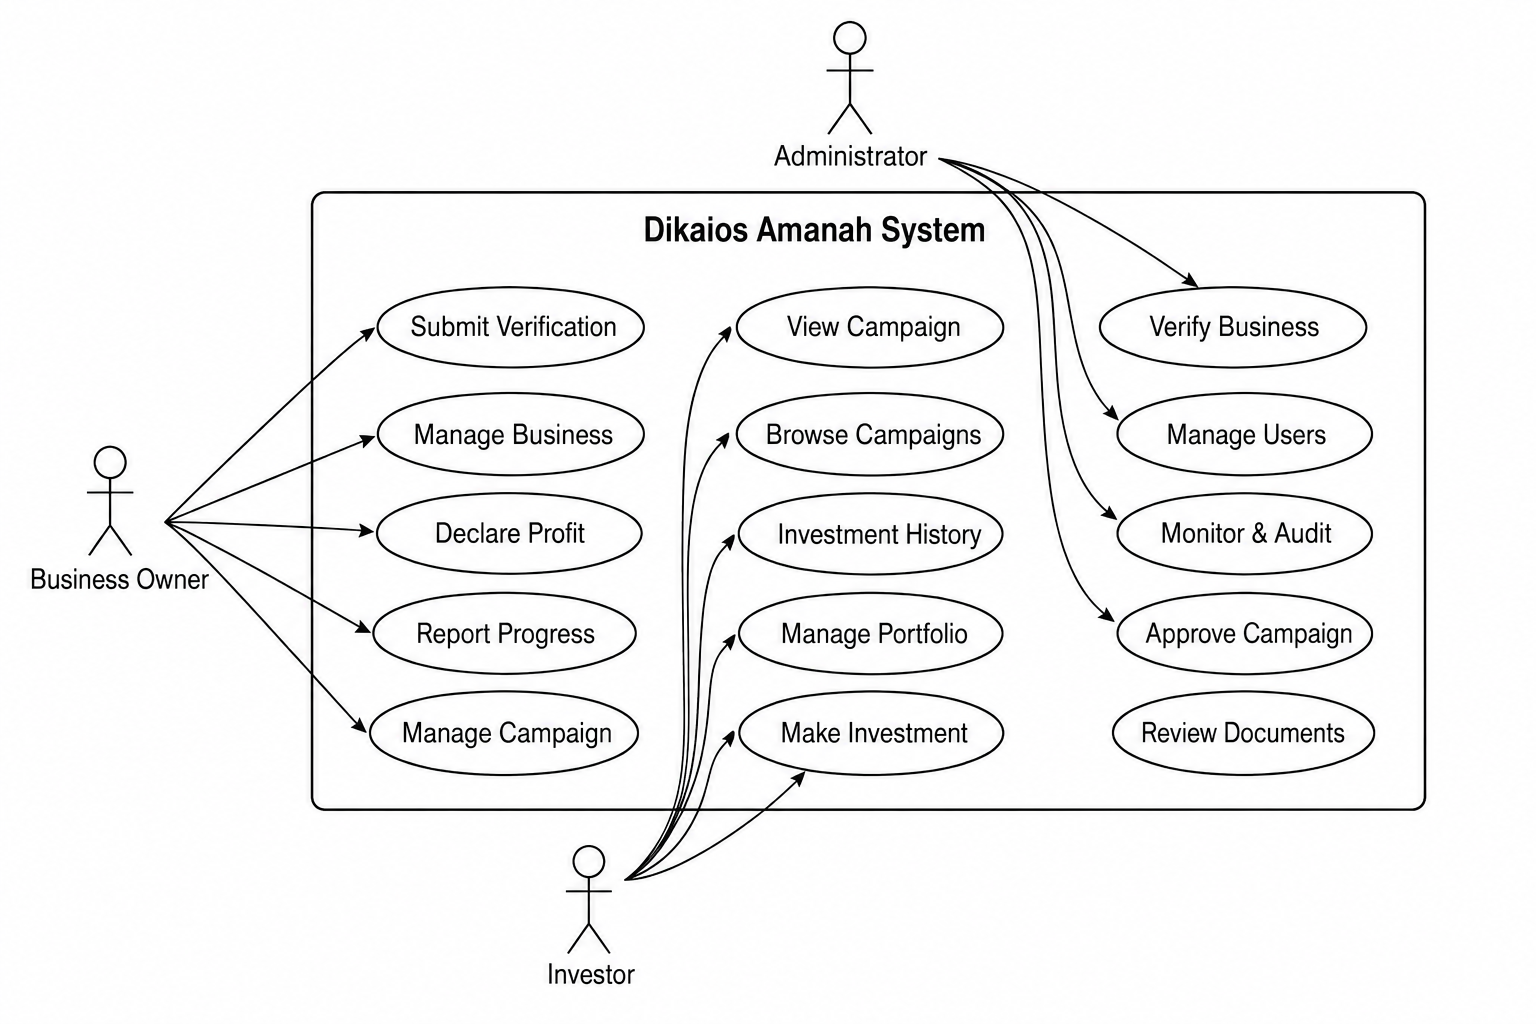
\includegraphics[width=\textwidth]{images/use_case.png}
    \caption{Dikaios Amanah Use Case Diagram}
    \label{fig:use-case}
\end{figure}


% ============================================================
% BUSINESS OWNER USE CASES
% ============================================================

\subsection{Business Owner Use Cases}

The Business Owner interacts with the system primarily to establish a
verified business profile and obtain investment through Musharakah-based
campaigns.

\subsubsection{Register and Authenticate}

The Business Owner creates an account and authenticates using the secure
authentication mechanism provided by the system.

\textbf{Precondition:}
The user does not already have an active account.

\textbf{Main Flow:}
\begin{enumerate}
    \item The Business Owner provides registration information.
    \item The system validates the submitted information.
    \item The system creates the user account.
    \item The Business Owner logs into the system.
    \item The system authenticates the credentials and provides access to the
    Business Owner dashboard.
\end{enumerate}

\textbf{Postcondition:}
The Business Owner is authenticated and can access authorized system
functions.


\subsubsection{Submit Business Verification}

The Business Owner submits business information and supporting documents for
administrative verification.

\textbf{Precondition:}
The Business Owner is authenticated.

\textbf{Main Flow:}
\begin{enumerate}
    \item The Business Owner enters business information.
    \item The Business Owner uploads the required documents.
    \item The system validates the submitted information.
    \item The system stores the verification record and documents.
    \item The system notifies the Administrator.
\end{enumerate}

\textbf{Postcondition:}
The business verification request is available for Administrator review.


\subsubsection{Create Investment Campaign}

A verified Business Owner creates an investment campaign containing the
required business and funding information.

\textbf{Precondition:}
The Business Owner and business have been verified.

\textbf{Main Flow:}
\begin{enumerate}
    \item The Business Owner selects the campaign creation function.
    \item The Business Owner provides campaign title and description.
    \item The Business Owner specifies the funding goal and related
    information.
    \item The system validates the information.
    \item The system creates the campaign.
\end{enumerate}

\textbf{Postcondition:}
The campaign is stored and can be made available to eligible investors.


\subsubsection{Monitor Investment Campaign}

The Business Owner monitors campaign status and funding progress.

\textbf{Main Flow:}
\begin{enumerate}
    \item The Business Owner opens the campaign dashboard.
    \item The system retrieves campaign information.
    \item The system displays current funding and campaign status.
\end{enumerate}


\subsubsection{Declare Profit}

The Business Owner submits profit information associated with an investment
campaign.

\textbf{Precondition:}
An applicable investment campaign exists.

\textbf{Main Flow:}
\begin{enumerate}
    \item The Business Owner selects the profit declaration function.
    \item The Business Owner enters the profit amount and reporting period.
    \item The system validates the submitted information.
    \item The system stores the profit declaration.
    \item The event is recorded in the audit layer.
\end{enumerate}

\textbf{Postcondition:}
The profit declaration is stored and available for authorized processing
and monitoring.


% ============================================================
% INVESTOR USE CASES
% ============================================================

\subsection{Retail Investor Use Cases}

Retail Investors interact with the system to discover verified investment
opportunities, participate in campaigns, and monitor their investments.

\subsubsection{Register and Complete Investor Verification}

The Retail Investor creates an account and provides the required information
for verification.

\textbf{Main Flow:}
\begin{enumerate}
    \item The Investor registers an account.
    \item The system validates the submitted information.
    \item The Investor provides required verification information.
    \item The system stores the verification information.
    \item The Administrator reviews the submitted information.
\end{enumerate}

\textbf{Postcondition:}
The Investor account is available according to its verification status.


\subsubsection{Browse Verified Businesses}

The Investor searches and views verified businesses available on the
platform.

\textbf{Main Flow:}
\begin{enumerate}
    \item The Investor opens the investment marketplace.
    \item The system retrieves eligible verified businesses.
    \item The system displays business profiles and available campaigns.
    \item The Investor selects a business or campaign for further review.
\end{enumerate}


\subsubsection{Review Investment Campaign}

The Investor reviews the information associated with an investment
opportunity before making an investment decision.

The system provides relevant campaign information, business information,
funding progress, and available investment details.


\subsubsection{Participate in Investment Campaign}

The Investor participates in an available Musharakah-based investment
campaign.

\textbf{Precondition:}
The Investor is authenticated and eligible to participate.

\textbf{Main Flow:}
\begin{enumerate}
    \item The Investor selects an available campaign.
    \item The Investor enters the intended investment amount.
    \item The system validates the investment information.
    \item The system records the investment.
    \item The investment status is updated.
    \item The event is recorded in the audit layer.
\end{enumerate}

\textbf{Postcondition:}
The investment appears in the Investor's portfolio.


\subsubsection{Monitor Investment Portfolio}

The Investor monitors investment status and portfolio information.

\begin{enumerate}
    \item The Investor opens the portfolio dashboard.
    \item The system retrieves investment records.
    \item The system displays investment status and relevant portfolio
    information.
\end{enumerate}


% ============================================================
% ADMINISTRATOR USE CASES
% ============================================================

\subsection{Administrator Use Cases}

The Administrator is responsible for verification, approval, monitoring,
and administrative control of the platform.

\subsubsection{Review Business Verification}

The Administrator reviews submitted business verification requests.

\textbf{Main Flow:}
\begin{enumerate}
    \item The Administrator opens the pending verification list.
    \item The system retrieves the submitted verification information.
    \item The Administrator reviews business information and documents.
    \item The Administrator approves or rejects the verification request.
    \item The system updates the verification status.
    \item The system records the decision in the audit layer.
    \item The Business Owner is notified of the result.
\end{enumerate}


\subsubsection{Manage Users}

The Administrator manages authorized users and their system status.

Possible administrative actions include reviewing user information,
updating account status, and managing access according to the user's role.


\subsubsection{Monitor System Activity}

The Administrator reviews system activity and important operational events.

The system provides activity records generated by important actions such as
verification decisions, investment activities, and other critical operations.


\subsubsection{Review Audit Records}

The Administrator reviews audit records generated by the Permissioned Trust
and Audit Layer.

Audit records provide tamper-evident evidence of important system events and
support accountability and transparency.


% ============================================================
% USE CASE SUMMARY
% ============================================================

\subsection{Use Case Summary}

\begin{table}[H]
\centering
\caption{Dikaios Amanah Use Case Summary}
\label{tab:use-case-summary}
\begin{tabularx}{\textwidth}{>{\raggedright\arraybackslash}p{0.22\textwidth}
>{\raggedright\arraybackslash}p{0.22\textwidth}
X}
\toprule
\textbf{Actor} & \textbf{Use Case} & \textbf{Description} \\
\midrule

Business Owner &
Register and Authenticate &
Creates an account and securely accesses the platform. \\

Business Owner &
Submit Business Verification &
Submits business information and supporting documents for verification. \\

Business Owner &
Create Investment Campaign &
Creates a Musharakah-based investment campaign. \\

Business Owner &
Monitor Campaign &
Monitors campaign status and funding progress. \\

Business Owner &
Declare Profit &
Submits profit information for an investment campaign. \\

Retail Investor &
Register and Verify &
Creates an account and completes required verification. \\

Retail Investor &
Browse Businesses &
Views verified businesses and available opportunities. \\

Retail Investor &
Review Campaign &
Examines investment campaign information before investing. \\

Retail Investor &
Participate in Investment &
Records participation in an eligible investment campaign. \\

Retail Investor &
Monitor Portfolio &
Views investment status and portfolio information. \\

Administrator &
Review Verification &
Reviews business information and supporting documents. \\

Administrator &
Manage Users &
Manages user accounts and access status. \\

Administrator &
Monitor Activity &
Reviews important platform activities. \\

Administrator &
Review Audit Records &
Reviews tamper-evident records of critical system events. \\

\bottomrule
\end{tabularx}
\end{table}


% ============================================================
% SEQUENCE DIAGRAM
% ============================================================

\subsection{Business Verification Sequence}

The sequence diagram describes the interaction between the Business Owner,
Administrator, web interface, backend API, verification service, database,
audit service, and notification service during business verification.

\begin{figure}[H]
    \centering
    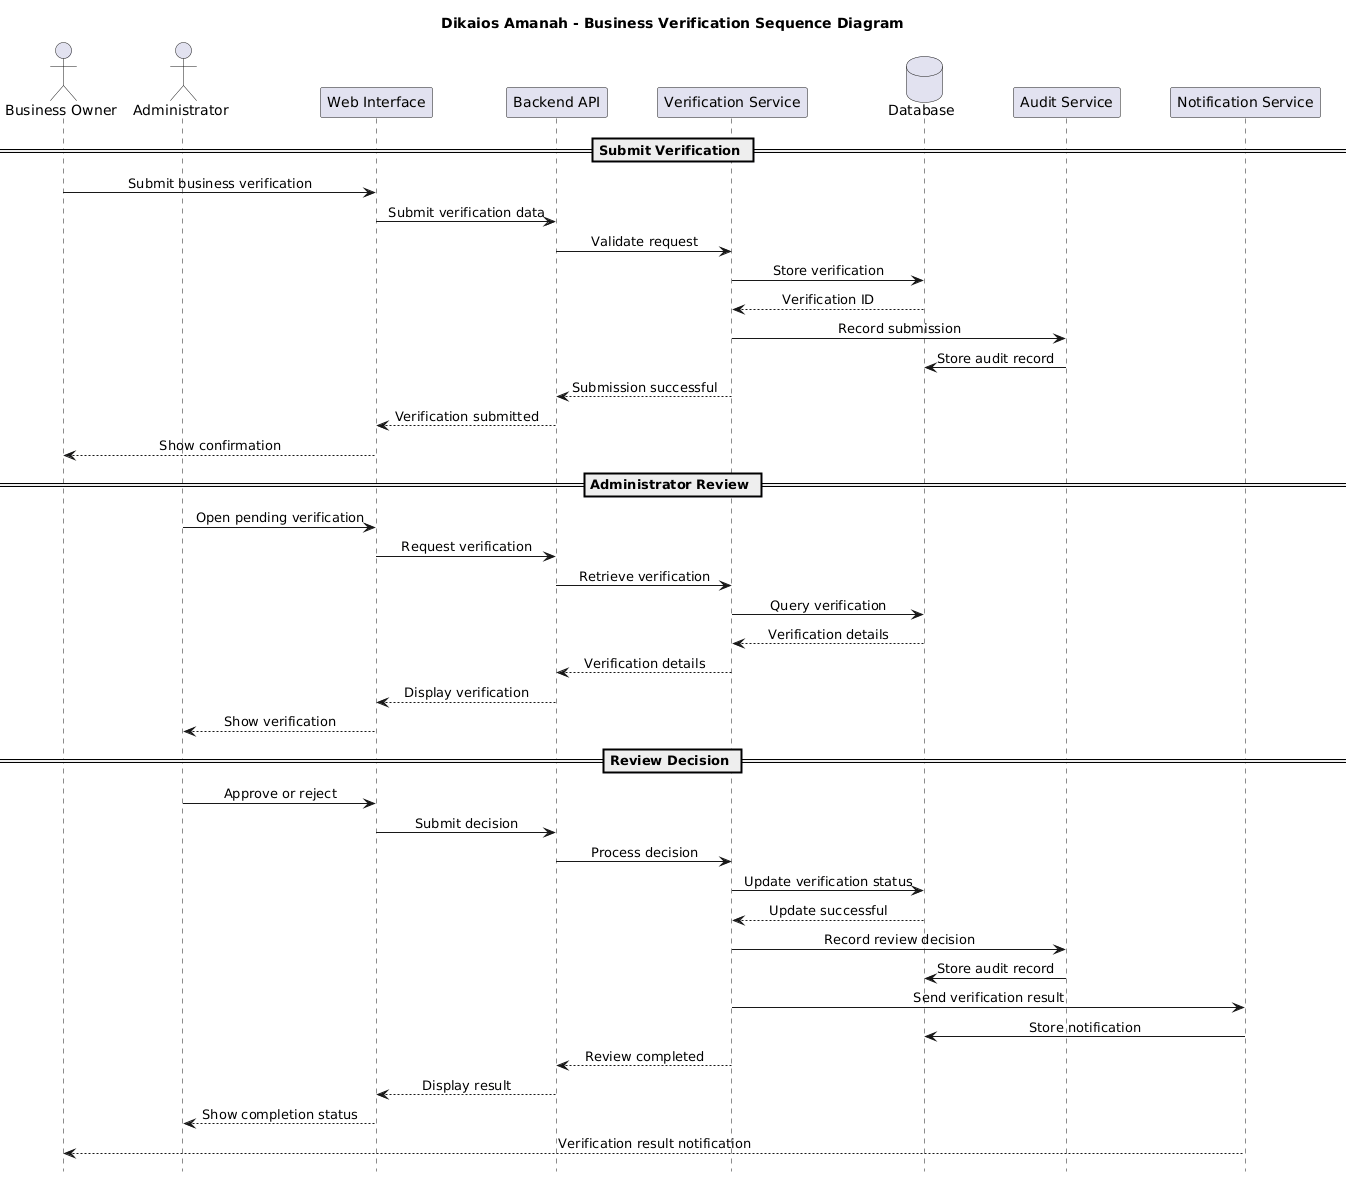
\includegraphics[width=\textwidth]{images/sequence_diagram.png}
    \caption{Business Verification Sequence Diagram}
    \label{fig:sequence-diagram}
\end{figure}


% ============================================================
% ACTIVITY DIAGRAM
% ============================================================

\subsection{Business Verification Activity}

The activity diagram illustrates the workflow beginning with business
information submission and continuing through validation, administrative
review, approval or rejection, and notification.

\begin{figure}[H]
    \centering
    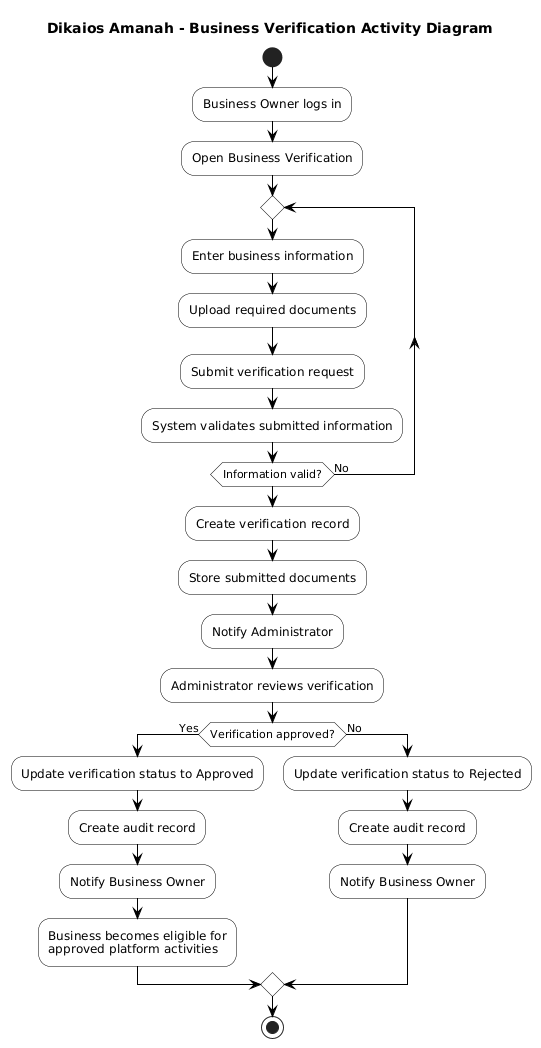
\includegraphics[width=0.85\textwidth]{images/activity_diagram.png}
    \caption{Business Verification Activity Diagram}
    \label{fig:activity-diagram}
\end{figure}


% ============================================================
% CLASS DIAGRAM
% ============================================================

\subsection{System Class Structure}

The class diagram presents the principal entities involved in the Dikaios
Amanah system, including users, business owners, administrators, businesses,
campaigns, investments, verifications, documents, profit declarations,
notifications, and audit records.

\begin{figure}[H]
    \centering
    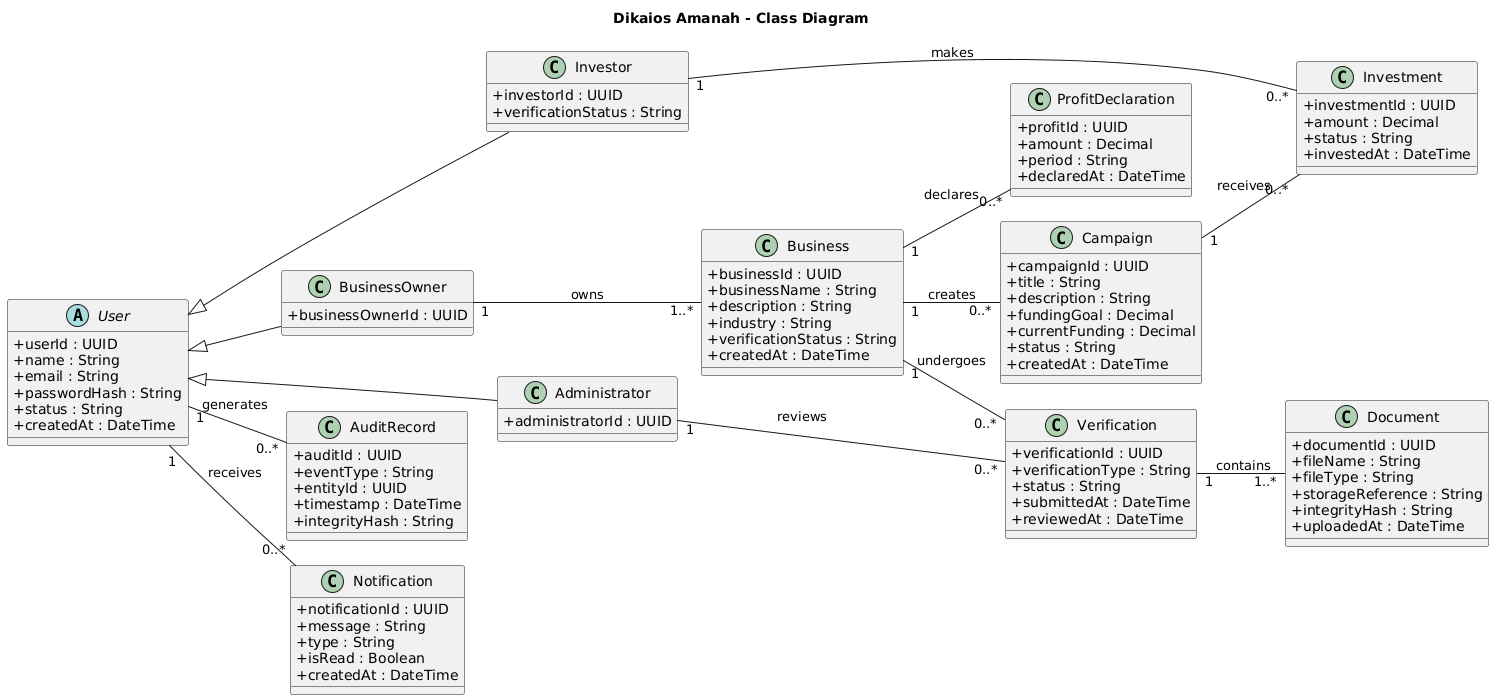
\includegraphics[width=\textwidth]{images/class_diagram.png}
    \caption{Dikaios Amanah Class Diagram}
    \label{fig:class-diagram}
\end{figure}


% ============================================================
% COMPONENT DIAGRAM
% ============================================================

\subsection{System Component Structure}

The component diagram presents the major software components of the proposed
Dikaios Amanah architecture and their relationships with the application
database and document storage.

\begin{figure}[H]
    \centering
    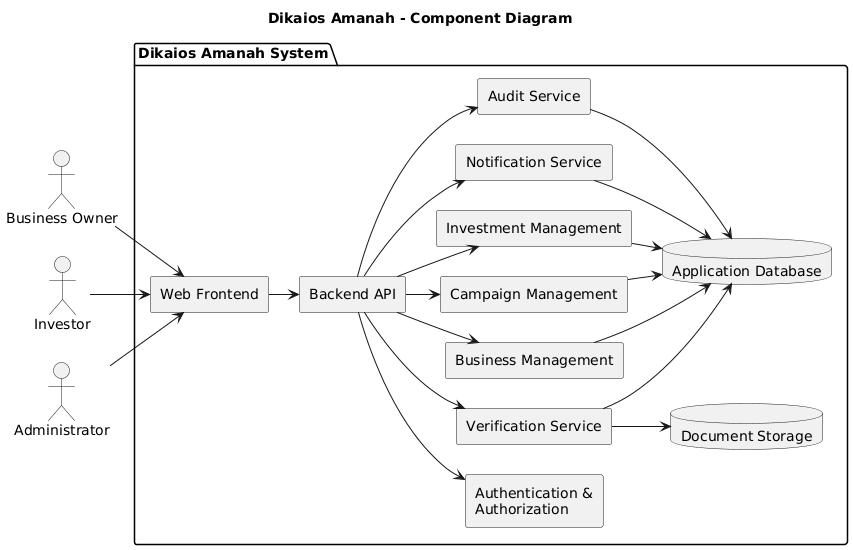
\includegraphics[width=\textwidth]{images/component_diagram.png}
    \caption{Dikaios Amanah Component Diagram}
    \label{fig:component-diagram}
\end{figure}


% ============================================================
% FISHBONE / ISHIKAWA DIAGRAM
% ============================================================

\subsection{Problem Cause Analysis}

The Fishbone (Ishikawa) Diagram identifies the major causes contributing to
the central problem of lack of trust and transparency in small-business
investment.

The identified cause categories include Information, Verification,
Transparency, Security, Process, and Investor Awareness.

\begin{figure}[H]
    \centering
    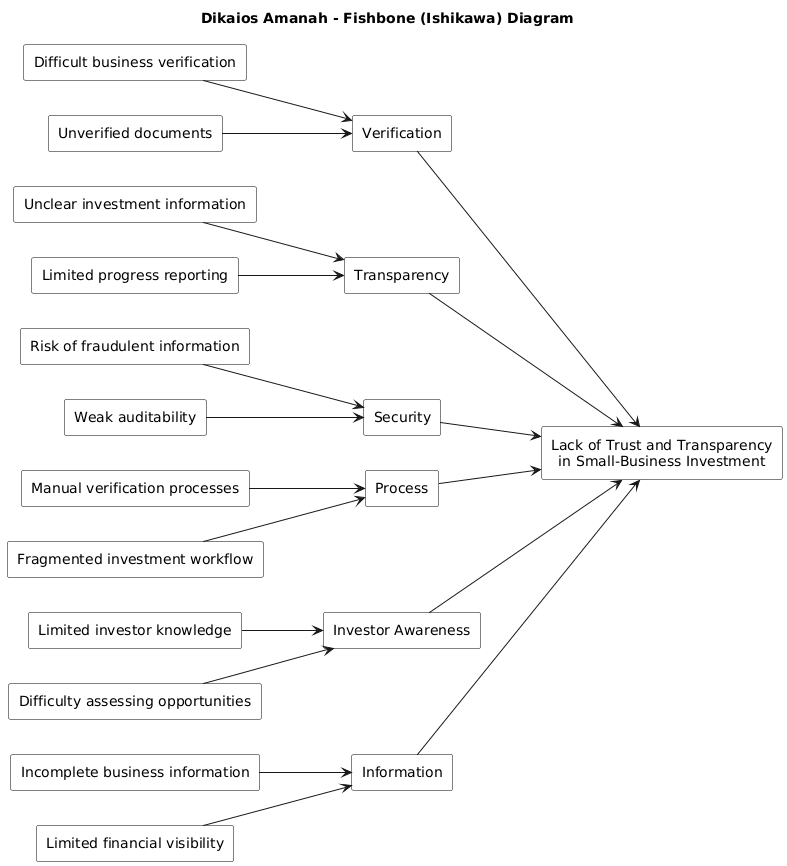
\includegraphics[width=\textwidth]{images/fishbone_diagram.png}
    \caption{Dikaios Amanah Fishbone (Ishikawa) Diagram}
    \label{fig:fishbone-diagram}
\end{figure}


% ============================================================
% RELATIONSHIP TO SYSTEM REQUIREMENTS
% ============================================================

\subsection{Relationship to System Requirements}

The identified use cases provide the functional foundation for subsequent
requirements specification and system design. They identify the primary
interactions that must be supported by the system and provide a basis for
deriving functional requirements, database entities, system workflows, and
software components.

The proposed system scope includes user authentication, business
verification, secure document management, investment campaign creation,
campaign browsing, investment tracking, portfolio management, profit
declaration, notifications, activity logging, and the Permissioned Trust
and Audit Layer.

}{}

% ====================================================
% 8. DATA REQUIREMENTS
% ====================================================

\IfFileExists{chapters/data_requirements.tex}{
    \section{Data Requirements}
    \subsection{Data Requirements}

The Dikaios Amanah system requires structured and reliable data to support
user management, business verification, investment campaign management,
investment participation, profit reporting, notifications, and system
auditing. The system shall store and manage the following major categories
of data.

\subsubsection{User Data}

The system shall maintain information required to identify and manage
registered users. User data shall include:

\begin{itemize}
    \item Unique user identifier
    \item Full name
    \item Email address
    \item Authentication credentials or securely stored password hash
    \item User role
    \item Account status
    \item Account creation date and time
\end{itemize}

The system shall distinguish between the primary user roles of Business
Owner, Investor, and Administrator.

\subsubsection{Business Data}

The system shall maintain information about businesses registered on the
platform. Business data shall include:

\begin{itemize}
    \item Unique business identifier
    \item Business name
    \item Business description
    \item Industry or business category
    \item Business ownership information
    \item Verification status
    \item Business registration information where applicable
    \item Creation and update timestamps
\end{itemize}

\subsubsection{Verification Data}

The system shall maintain information associated with business and user
verification processes. Verification data shall include:

\begin{itemize}
    \item Unique verification identifier
    \item Verification type
    \item Related business or user
    \item Verification status
    \item Submission date and time
    \item Review date and time
    \item Reviewing administrator
    \item Verification remarks where applicable
\end{itemize}

The system shall preserve the status of verification requests so that
authorized users can determine whether a verification request is pending,
approved, or rejected.

\subsubsection{Document Data}

The system shall maintain metadata associated with documents submitted
during verification. Document data shall include:

\begin{itemize}
    \item Unique document identifier
    \item Related verification record
    \item File name
    \item File type
    \item Storage reference
    \item Document integrity information where applicable
    \item Upload date and time
\end{itemize}

The system shall restrict access to verification documents according to
the user's authorization level.

\subsubsection{Investment Campaign Data}

The system shall maintain information about investment campaigns created
by verified businesses. Campaign data shall include:

\begin{itemize}
    \item Unique campaign identifier
    \item Related business
    \item Campaign title
    \item Campaign description
    \item Funding goal
    \item Current funding amount
    \item Campaign status
    \item Creation date and time
    \item Approval information where applicable
\end{itemize}

Only campaigns satisfying the required verification and approval
conditions shall be made available for participation.

\subsubsection{Investment Data}

The system shall maintain records of investment activities performed by
investors. Investment data shall include:

\begin{itemize}
    \item Unique investment identifier
    \item Related investor
    \item Related campaign
    \item Investment amount
    \item Investment status
    \item Investment date and time
\end{itemize}

For the scope of the academic project, investment activities represent
the system's simulated investment functionality rather than real-world
financial transactions.

\subsubsection{Profit Declaration Data}

The system shall maintain information submitted by businesses regarding
their declared profits. Profit declaration data shall include:

\begin{itemize}
    \item Unique profit declaration identifier
    \item Related business
    \item Declared profit amount
    \item Reporting period
    \item Declaration date and time
    \item Relevant status or review information where applicable
\end{itemize}

\subsubsection{Audit Data}

The system shall maintain audit records for significant system activities
to support transparency and accountability. Audit data shall include:

\begin{itemize}
    \item Unique audit record identifier
    \item User associated with the activity
    \item Event type
    \item Related entity identifier where applicable
    \item Date and time of the event
    \item Integrity information where applicable
\end{itemize}

Audit records shall be protected from unauthorized modification or
deletion.

\subsubsection{Notification Data}

The system shall maintain notification information for communicating
important system events to users. Notification data shall include:

\begin{itemize}
    \item Unique notification identifier
    \item Recipient user
    \item Notification type
    \item Notification message
    \item Read or unread status
    \item Creation date and time
\end{itemize}

\subsubsection{Data Integrity and Security Requirements}

The system shall maintain the integrity and confidentiality of stored
data. Sensitive information shall not be stored in plaintext where
secure storage mechanisms are required.

The system shall enforce appropriate access control so that users can
only access data permitted by their roles and responsibilities.

The system shall validate data submitted by users before storing it.
Required fields shall be checked for completeness, and invalid or
inconsistent data shall be rejected.

The system shall maintain appropriate timestamps for important records
to support traceability and auditing.

\subsubsection{Data Retention and Backup}

Important system records shall be retained for the duration required by
the project's operational and academic scope. The system design shall
allow appropriate backup and recovery mechanisms to be introduced for
persistent data.

As this project is developed as a Software Engineering Lab project,
production-level financial data retention and regulatory requirements are
outside the current implementation scope.
}{}

% ====================================================
% 9. SYSTEM CONSTRAINTS AND LIMITATIONS
% ====================================================

\IfFileExists{chapters/constraints.tex}{
    \section{System Constraints and Limitations}
    \subsection{System Constraints and Limitations}

The development and operation of the Dikaios Amanah system are subject
to several technical, operational, security, and project-level
constraints. These constraints define the boundaries of the proposed
system and its implementation within the scope of the Software
Engineering Lab project.

\subsubsection{Project Scope Constraint}

Dikaios Amanah is developed as an academic Software Engineering Lab
project. Therefore, the system is intended to demonstrate the proposed
software architecture, functionality, security concepts, and workflow
rather than operate as a production financial platform.

Production-scale deployment, commercial operation, and regulatory
certification are outside the current project scope.

\subsubsection{Financial Transaction Limitation}

The investment functionality implemented within the project represents
simulated investment activities. The system does not process real
financial transactions, transfer real funds, or provide actual
investment services.

Any financial values displayed by the system are intended for
demonstration and testing purposes.

\subsubsection{Regulatory and Legal Constraints}

A production implementation of a platform involving investment
activities would be subject to applicable financial, business,
data-protection, and other regulatory requirements.

Obtaining licenses, regulatory approvals, legal certifications, and
formal authorization to operate a financial service are outside the
scope of this academic project.

\subsubsection{Third-Party Service Dependency}

The system may depend on external services for hosting, cloud
infrastructure, file storage, authentication, email or notification
delivery, and other supporting functionality.

Availability, pricing, service limits, and changes to third-party
services may affect system operation.

\subsubsection{Internet and Infrastructure Dependency}

The web-based system requires network connectivity for communication
between the client application, backend services, database, and
supporting cloud infrastructure.

Temporary network failures or service outages may prevent users from
accessing certain system functionality.

\subsubsection{Document Verification Limitation}

The system can collect and manage documents submitted for verification,
but the academic implementation cannot guarantee that submitted
documents are legally authentic.

Document review and verification functionality is intended to
demonstrate the software workflow and access-control mechanisms rather
than replace formal legal or governmental verification procedures.

\subsubsection{Security Constraints}

The system shall implement appropriate authentication, authorization,
input validation, secure credential handling, and audit mechanisms
within the project's technical scope.

However, the academic implementation cannot guarantee complete
protection against every possible cybersecurity threat. Production-level
penetration testing, security certification, continuous security
monitoring, and advanced threat detection are outside the current
scope.

\subsubsection{Scalability Constraint}

The initial implementation is designed for demonstration and academic
evaluation rather than large-scale commercial usage.

The system may therefore require additional infrastructure,
optimization, caching, database scaling, and load-balancing mechanisms
before supporting a large number of concurrent users.

\subsubsection{Data Availability Constraint}

The quality of system demonstrations and testing depends on the
availability of suitable test data.

The project may use controlled, synthetic, or sample data for
demonstration purposes. Real confidential business, financial, or
personal information shall not be required for the academic
implementation.

\subsubsection{Development Resource Constraint}

The project is developed within the time, hardware, software, and
resource limitations of an academic Software Engineering Lab project.

These limitations may restrict the number of advanced features that can
be implemented during the project period.

\subsubsection{Deployment Constraint}

The final system may be deployed using cloud-based infrastructure
appropriate for the project's requirements. However, the deployment
configuration is intended for demonstration and evaluation and may not
provide the redundancy, monitoring, disaster recovery, and operational
support expected from a production financial platform.
}{}

% ====================================================
% 10. FUTURE ENHANCEMENTS
% ====================================================

\IfFileExists{chapters/future_enhancements.tex}{
    \section{Future Enhancements}
    \subsection{Future Enhancements}

The current Dikaios Amanah system is designed as an academic MVP.
Several features and improvements can be considered for future versions
if the system is extended beyond the scope of the Software Engineering
Lab project.

\subsubsection{Real Financial Transaction Integration}

A future production-oriented version could integrate with authorized
financial institutions or payment service providers to support real
financial transactions.

Such functionality would require appropriate regulatory approval,
security controls, financial compliance mechanisms, and integration with
authorized payment infrastructure.

\subsubsection{Advanced Business Verification}

The verification system could be extended to integrate with official
business registries and authorized verification services.

Automated verification could reduce manual review requirements and
improve the reliability and speed of the verification process.

\subsubsection{Advanced Risk Assessment}

Future versions could introduce more sophisticated risk assessment
mechanisms using historical business performance, financial indicators,
market information, and other relevant factors.

Machine learning techniques could also be investigated to assist with
risk classification and decision support.

\subsubsection{Enhanced Fraud Detection}

The system could be extended with automated fraud detection mechanisms
to identify suspicious accounts, unusual investment patterns, document
inconsistencies, and other potentially fraudulent activities.

\subsubsection{Mobile Application}

A dedicated mobile application could be developed to provide Business
Owners, Investors, and Administrators with convenient access to the
platform through mobile devices.

\subsubsection{Advanced Notification System}

Future versions could support multiple notification channels, including
email, SMS, and push notifications, for important verification,
campaign, investment, and administrative events.

\subsubsection{Improved Scalability}

The system could be expanded to support larger numbers of users and
higher transaction volumes through additional infrastructure,
database optimization, caching, load balancing, and distributed
services.

\subsubsection{Enhanced Analytics and Reporting}

Advanced dashboards and reporting capabilities could be introduced to
provide Business Owners, Investors, and Administrators with more
detailed insights into business performance, campaign progress,
investment activity, and platform activity.

\subsubsection{Expanded Trust and Audit Infrastructure}

The Permissioned Trust and Audit Layer could be expanded to provide
stronger tamper-evident record keeping and more comprehensive audit
capabilities for critical system events.

\subsubsection{Regulatory and Production Readiness}

If the system were developed beyond the academic environment, future
work would include formal security assessment, regulatory compliance,
privacy controls, operational monitoring, disaster recovery, and other
requirements necessary for production deployment.
}{}

% ====================================================
% 11. TESTING REQUIREMENTS
% ====================================================

\IfFileExists{chapters/testing_requirements.tex}{
    \section{Testing Requirements}
    \subsection{Testing Requirements}

Testing shall be performed to verify that Dikaios Amanah satisfies its
functional and non-functional requirements. The testing process shall
focus on the correctness of the major system workflows, role-based
access control, data validation, security mechanisms, and system
integration.

\subsubsection{Unit Testing}

Individual software components and functions shall be tested
independently to verify that they produce the expected results.

Unit testing should cover important backend services, validation
functions, authentication-related functions, and other critical
application logic.

\subsubsection{Integration Testing}

Integration testing shall verify that different system components
communicate correctly.

The following integrations shall be considered:

\begin{itemize}
    \item Frontend and backend API communication.
    \item Backend and PostgreSQL database communication.
    \item Backend and document storage.
    \item Authentication and authorization services.
    \item Backend and the trust and audit layer.
\end{itemize}

\subsubsection{System Testing}

System testing shall evaluate the complete application as an integrated
system.

Testing shall cover the major workflows of Business Owners, Investors,
and Administrators, including business verification, campaign
management, investment simulation, profit declaration, and administrative
operations.

\subsubsection{Functional Testing}

Functional tests shall verify that the implemented system behavior
matches the functional requirements.

Representative functional test cases shall include:

\begin{itemize}
    \item User registration and login.
    \item Role-based access control.
    \item Business profile creation and management.
    \item Business verification submission.
    \item Document upload and management.
    \item Campaign creation and approval.
    \item Campaign browsing.
    \item Simulated investment.
    \item Portfolio and investment history.
    \item Profit declaration.
    \item Administrative review and monitoring.
    \item Audit record generation.
\end{itemize}

\subsubsection{Security Testing}

Security testing shall verify that protected system resources cannot be
accessed by unauthorized users.

Security testing shall include:

\begin{itemize}
    \item Authentication testing.
    \item Authorization and role testing.
    \item Invalid credential testing.
    \item Protected endpoint testing.
    \item Input validation testing.
    \item Unauthorized document access testing.
    \item Session or token validation testing.
\end{itemize}

\subsubsection{Usability Testing}

Usability testing shall evaluate whether users can understand and
complete the major system workflows using the provided interface.

The primary user roles shall be considered during usability testing,
including Business Owners, Investors, and Administrators.

\subsubsection{Performance Testing}

Basic performance testing shall be performed to evaluate the system's
response under representative academic testing conditions.

Testing may include:

\begin{itemize}
    \item API response time.
    \item Page loading behavior.
    \item Database query performance.
    \item Response behavior under multiple simulated requests.
\end{itemize}

Production-scale load and stress testing are outside the current
academic project scope.

\subsubsection{Negative Testing}

The system shall be tested with invalid, incomplete, or unexpected input
to verify that errors are handled appropriately.

Examples include:

\begin{itemize}
    \item Invalid login credentials.
    \item Missing required fields.
    \item Invalid document types.
    \item Invalid investment amounts.
    \item Unauthorized operations.
    \item Invalid campaign information.
\end{itemize}

\subsubsection{User Acceptance Testing}

User Acceptance Testing (UAT) shall verify that the system satisfies
the expected workflows from the perspective of its intended users.

Representative scenarios shall be executed for the Business Owner,
Investor, and Administrator roles.

\subsubsection{Test Documentation}

Test cases shall document the following information where applicable:

\begin{itemize}
    \item Test case identifier.
    \item Related requirement.
    \item Test objective.
    \item Preconditions.
    \item Test input.
    \item Expected result.
    \item Actual result.
    \item Test status.
\end{itemize}

Test results shall be used to identify defects and verify that corrective
changes satisfy the corresponding requirements.
}{}

% ====================================================
% 12. REQUIREMENTS TRACEABILITY
% ====================================================

\IfFileExists{chapters/traceability.tex}{
    \section{Requirements Traceability}
    \subsection{Requirements Traceability}

Requirements traceability establishes a relationship between the
identified system requirements, their implementation, and the testing
activities used to verify them.

The traceability process helps ensure that each major requirement is
addressed by the system design and can be verified through appropriate
testing.

\subsubsection{Traceability Approach}

Each functional requirement shall have a unique identifier. These
identifiers shall be used consistently throughout the system design,
implementation, and testing documentation.

The main traceability relationship is:

\begin{center}
\textbf{Requirement $\rightarrow$ Design $\rightarrow$ Implementation
$\rightarrow$ Test Case}
\end{center}

This approach allows the development team to determine whether a
requirement has been implemented and whether sufficient testing has been
performed.

\subsubsection{Functional Requirement Traceability}

The following table provides a high-level mapping between the major
functional requirements and their corresponding system areas and testing
activities.

\begin{table}[H]
\centering
\small

\begin{tabularx}{\textwidth}{>{\bfseries}l X X X}
\toprule
Requirement & System Area & Design Element & Verification \\
\midrule

FR-AUTH &
Authentication and account management &
Authentication module &
Authentication tests \\

FR-BO &
Business Owner functionality &
Business management and campaign modules &
Business Owner functional tests \\

FR-INV &
Investor functionality &
Investment and portfolio modules &
Investor functional tests \\

FR-ADM &
Administrator functionality &
Administration module &
Administrator functional tests \\

FR-VER &
Business verification &
Verification and document modules &
Verification test cases \\

FR-CAM &
Campaign management &
Campaign module &
Campaign functional tests \\

FR-INVEST &
Investment functionality &
Investment module &
Investment test cases \\

FR-PROFIT &
Profit declaration &
Profit management module &
Profit declaration tests \\

FR-AUDIT &
Audit and traceability &
Audit and Trust Layer &
Audit verification tests \\

\bottomrule
\end{tabularx}

\caption{High-Level Functional Requirement Traceability}
\label{tab:functional_traceability}

\end{table}

\subsubsection{Non-Functional Requirement Traceability}

Non-functional requirements shall also be considered during system
design and testing.

\begin{table}[H]
\centering
\small

\begin{tabularx}{\textwidth}{>{\bfseries}l X X}
\toprule
Requirement & Related System Area & Verification Method \\
\midrule

Security &
Authentication, authorization, input validation &
Security testing \\

Performance &
Backend, database, and frontend &
Performance testing \\

Usability &
User interface &
Usability testing \\

Reliability &
Application and database services &
System and integration testing \\

Maintainability &
Software architecture and modular components &
Code and architecture review \\

\bottomrule
\end{tabularx}

\caption{Non-Functional Requirement Traceability}
\label{tab:nonfunctional_traceability}

\end{table}

\subsubsection{Traceability During Development}

The traceability information shall be maintained throughout the
development process. Changes to important requirements should be
reflected in the relevant design components, implementation tasks, and
test cases.

This approach will help reduce the possibility of implementing system
features that cannot be traced back to an identified requirement and
will support systematic verification of the final system.
}{}

% ====================================================
% REFERENCES
% ====================================================

\newpage

\section*{References}
\addcontentsline{toc}{section}{References}

\begin{enumerate}

\item Meta, ``React Documentation.'' Available:
\url{https://react.dev}

\item Node.js Foundation, ``Node.js Documentation.'' Available:
\url{https://nodejs.org}

\item Express.js, ``Express.js Documentation.'' Available:
\url{https://expressjs.com}

\item PostgreSQL Global Development Group, ``PostgreSQL Documentation.''
Available:
\url{https://www.postgresql.org/docs/}

\item Google, ``Firebase Documentation.'' Available:
\url{https://firebase.google.com/docs}

\item Auth0, ``JSON Web Token Introduction.'' Available:
\url{https://jwt.io/introduction}

\item NIST, ``Secure Hash Standard, FIPS PUB 180-4.'' Available:
\url{https://csrc.nist.gov/publications/detail/fips/180/4/final}

\item Hyperledger Foundation, ``Hyperledger Fabric Documentation.''
Available:
\url{https://hyperledger-fabric.readthedocs.io}

\item GitHub, ``GitHub Documentation.'' Available:
\url{https://docs.github.com}

\item Bangladesh Bank, ``SME Financing.'' Available:
\url{https://www.bb.org.bd}

\item SME Foundation Bangladesh, ``SME Development in Bangladesh.''
Available:
\url{https://www.smef.gov.bd}

\item AAOIFI, ``Shariah Standards.'' Available:
\url{https://aaoifi.com}

\end{enumerate}

% ====================================================

\end{document}